\documentclass[12pt]{article}
\usepackage{sbc-template}
\usepackage[alf]{abntex2cite} 
\usepackage{graphicx,url}
\usepackage[utf8]{inputenc}
\usepackage[brazil]{babel}
\usepackage{framed}                 %Incluindo Caixas
\usepackage{enumitem}               %Usando enumeraded
%\usepackage[latin1]{inputenc}      %Erro no inputenc.

\sloppy

\title{Um breve estudo sobre o Design Emocional: \\ contribuições e pesquisas em aberto}

\author{Alexandre Mendonça Fava\inst{1}}

\address{\inst{}Universidade do Estado de Santa Catarina - UDESC\\Programa de Pós-graduação em Computação Aplicada - PPGCA\\Joinville - SC - Brasil CEP: 89.219-710
    \email{\{alexandre.fava@hotmail.com\}}
}

\begin{document} 

\maketitle

\begin{abstract}
The emotions are present in both humans and animals. The manifestations of joy or sadness are a powerful feedback to understand if any action should be continued or interrupted. Some computational artifacts are based on some searches in the area of Emotional Design to build products that provide a better experience for users. In these cases, emotions such as joy, happiness and motivation are the most desired for the products. This article show some of these solutions and some open research in the area of Emotional Design.
\end{abstract} 


\begin{resumo} 
As emoções estão presentes tanto em seres humanos quanto em animais. As manifestações de alegria ou tristeza são um feeback para se compreender se uma determinada ação deve ser continuada ou interrompida. Alguns artefatos computacionais se baseiam em alguns achados na área do Design Emocional para construir produtos que proporcionem melhores experiência aos usuários, onde emoções como alegria, felicidade e motivação são as mais almejadas para os produtos. O presente artigo relata algumas destas soluções e lista algumas pesquisas em aberto na área do Desing Emocional.
\end{resumo}


\section{Introdução}\label{secao:introducao}

As emoções possuem impacto significativo no comportamento das pessoas. As emoções também são responsáveis por influenciar na percepção que determinados indivíduos tem do mundo e de objetivos. Na área comportamental já é sabido que a raiva de motoristas jovens no trânsito é um fator que implica diretamente em uma direção mais imprudente e arriscada \cite{zhang2016association}. No outro sentido, a compreensão da influência das emoções no comportamento humano é algo inclusive já  explorado por agências de publicidade \cite{preece2015interaction}.

Existem muitas aplicações em potencial para o uso da detecção automática de emoções em ambientes como a saúde, educação e até mesmo o trânsito. Um artefato vestível ou um sistema de reconhecimento facial, poderia identificar traços de raiva de um motorista ao volante, onde atitudes seriam tomadas de modo a minimizar eventuais ações imprudentes do condutor. 

A área da interação emocional preocupa-se com o que faz as pessoas se sentirem felizes, tristes, irritadas, ansiosas, frustradas ou motivadas. Para detectar as emoções nas pessoas automaticamente existem inúmeras técnicas, indo desde movimentos corporais, reconhecimento facial até diagnósticos cardíacos. 

A compreensão das emoções é um fator determinante na construção de artefatos computacionais mais amigáveis que proporcionem melhores experiências aos usuários \cite{preece2015interaction}. Neste campo cita-se, a computação afetiva, o design emocional e demais esferas da área de Iteração Humano-Computador (IHC).

O estudo das emoções do ponto de vista computacional está em constante crescimento, estando em vários contextos integrado com a Inteligência Artificial (IA) para a predição das emoções. O foco principal dos estudos está em como projetar produtos interativos para evocar certos tipos de respostas emocionais nas pessoas.  

O Design Emocional pretende associar a estética e funcionalidade de modo a conceber um produto que apele às emoções subjetivas do consumidor. A aparência é um dos fatores chaves desta área. A compreensão do impacto das cores e de certos tipos de formas ou traços no emocional das pessoas permite o desenvolvimento de sistemas e produtos mais chamativos e atrativos aos consumidores.

Tendo em vista a importância das emoções no comportamento e nas atitudes dos indivíduos, o presente artigo se presa a fornecer uma breve compilação de alguns resultados promissores na área do Design Emocional. Algumas pesquisas em aberto na área em questão também são abordadas pelo presente trabalho. Além de toda uma fundamentação teórica sobre o assunto, para uma compreensão mais apuradas de alguns conceitos abordados pelas pesquisas citadas. 

O presente artigo se secciona da seguinte maneira. A seção \ref{secao:fundamentacao} apresenta a fundamentação teórica no que diz respeito a alguns modelos da área do Design Emocional. A seção \ref{secao:trabalhos} lista alguns trabalho colhidos na temática em questão. A seção \ref{secao:desenvolvimento} exibe alguns pesquisas futuras em aberto na área e por fim a seção \ref{secao:conclusao} dá a conclusão da atual pesquisa. 


\section{Fundamentação}\label{secao:fundamentacao}

A compreensão de como as emoções funcionam fornece um alicerce estável para se projetar experiências mais agradáveis ao usuário. Uma vez que o contexto de uso esteja delimitado e seus constructos bem fundamentados é possível se ter um maior domínio sobre como um determinado produto irá desencadear efeitos ou reflexões ao usuário. Existem várias visões que fundamentam determinados conceitos no Design Emocional. A presente seção se limita a apresentar um pequeno leque dos modelos propostos na área de maior abrangência.  
 
\citeonline{norman2005emotional} definiu um modelo baseado em níveis que relaciona emoção e comportamento. O nível mais baixo (visceral), se objetiva a responder automaticamente a eventos que acontecem no mundo físico. O nível intermediário (comportamental), diz respeito aos processos cerebrais que controlam o comportamento cotidiano. Já o nível mais alto (reflexivo), se relaciona a contemplação. Todos os níveis podem ser observados na Figura \ref{fig:ModeloNorman}.

\begin{figure}[ht]
\centering
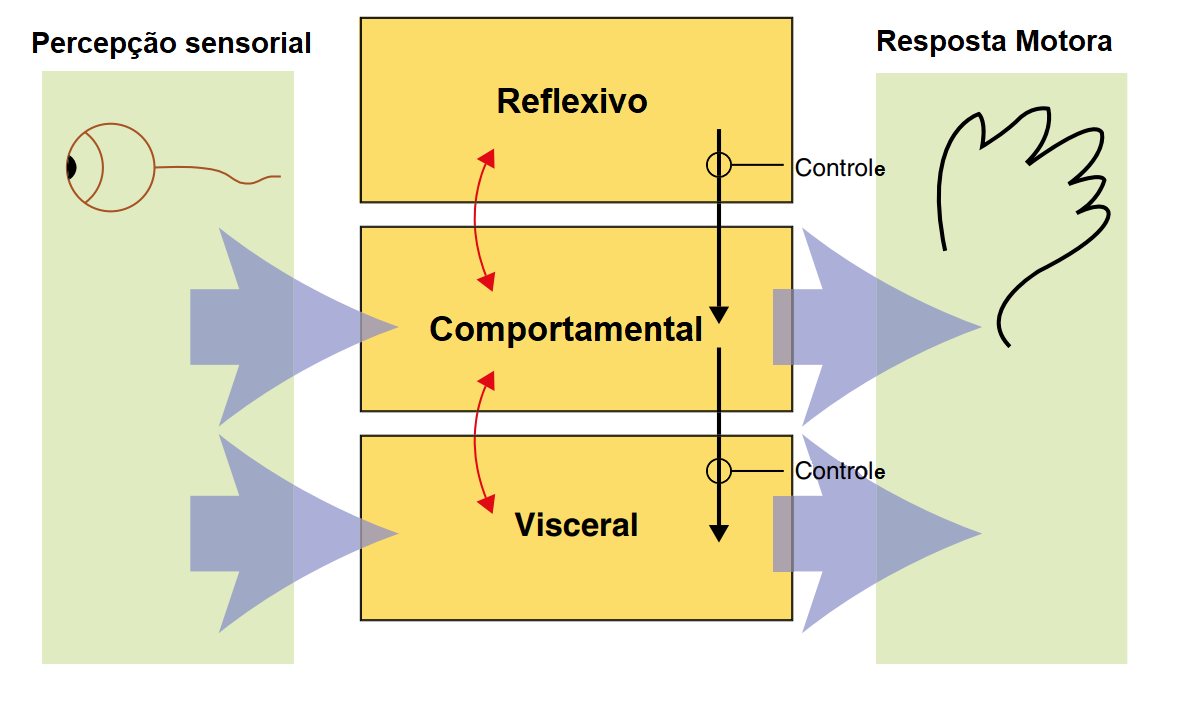
\includegraphics[width=1.15\textwidth]{Figuras/ModeloNorman.png}
\caption{Adaptado de \citeonline{norman2005emotional}}
\label{fig:ModeloNorman}
\end{figure}

O nível visceral responde rapidamente, fazendo julgamentos sobre o que é bom ou ruim, seguro ou perigoso, prazeroso ou abominável. As emoções associadas a este nível são:  medo, alegria, raiva e tristeza. O nível reflexivo envolve o pensamento consciente, onde as pessoas generalizam os eventos ou se afastam de suas rotinas diárias, enquanto que no nível comportamental é o local onde a maioria das atividades humanas ocorre.

O design visceral refere-se a fazer com que os produtos pareçam, sintam e tenham um bom som. O design comportamental é sobre uso e equivale aos valores tradicionais de usabilidade. O design reflexivo consiste em considerar o significado e o valor pessoal de um produto em uma cultura específica.

Outro modelo da área de Design Emocional é o proposto de \citeonline{desmet2009special}. São quatro formas que definem neste modelo como o design deve ser construído com foco nas emoções, sendo: 

\begin{enumerate}[label=(\alph*)]
\item Com foco no usuário: envolve o usuário no projeto, e suas emoções são o foco do processo de design. Técnicas exploratórias são comumente empregadas, inclusive colagens, mock-ups, entre outras. 
\item Com foco no designer: designers atuam como autores e, mais que gratificar usuários, esses profissionais desafiam os consumidores, apresentando algo diferenciado. 
\item Com foco em pesquisa: as diretrizes projetuais são frutos de pesquisa e/ou são testadas com usuários, comumente empregando técnicas de mensuração. 
\item Com foco em teoria: a teoria auxilia a qualificar o design em termos de impacto emocional. Nessa visão, insights teóricos ajudam a desenvolver conceitos.
\end{enumerate}

\newpage

\section{Estado da Arte}\label{secao:trabalhos}

Há inúmeros estudos relacionando o comportamento das pessoas a suas emoções. A atual seção apresenta uma revisão da literatura realizada para se obter a compreensão geral do Design Emocional.

\citeonline{carvalho2013design} analisaram o Duolingo, um site de aprendizagem de idiomas. Já na Homepage do site são notados os elementos que chamam mais a atenção dos usuários testados. A Figura \ref{fig:DuolingoHM} apresenta as regiões de maior visualização em comparação a Figura \ref{fig:Duolingo} que mostra a página inicial do Duolingo sem efeitos. 

\begin{figure}[h]
\centering
\begin{minipage}{.43\textwidth}
    \centering
    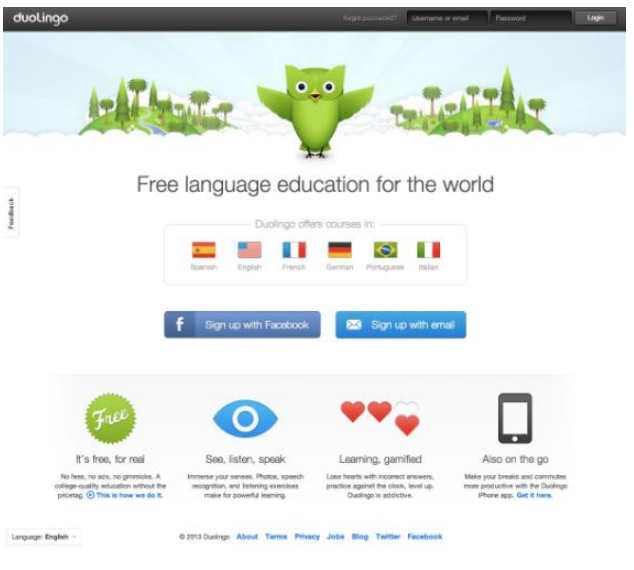
\includegraphics[width=\linewidth]{Figuras/Duolingo.png}
    \captionof{figure}{Página principal do Duolingo \cite{carvalho2013design}}
    \label{fig:Duolingo}
\end{minipage}%
\begin{minipage}{.48\textwidth}
    \centering
    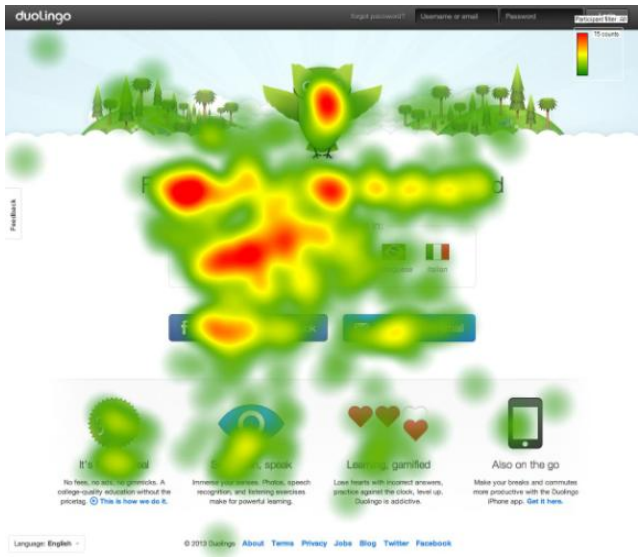
\includegraphics[width=\linewidth]{Figuras/DuolingoHM.png}
    \captionof{figure}{Mapa de Calor \cite{carvalho2013design}}
    \label{fig:DuolingoHM}
\end{minipage}
\end{figure}

Na Figura \ref{fig:DuolingoHM} é apresentado um mapa de calor (heatmap) que visa mostrar as regiões mais observadas por um grupo de usuário. Dentre as regiões mais observadas estão: as bandeiras dos cursos disponibilizados pelo Duolingo, o slogan do site, a mascote e o botão de registo do facebook; tendo sido fixados em primeiro lugar. A coleta deste tipo de informação é realizada com o auxílio do eye tracker, um dispositivo para mapear as zonas quentes de um página na web.

O heatmap mostra claramente um número elevado de fixações na mascote (a coruja verde). A literatura prévia da área já prevê que esse tipo de elemento gráfico chame a atenção de usuários e desperte emoções alegres. o foco na coruja está relacionado com algo chamado na literatura de baby-face bias; o qual corresponde as tendências em associar pessoas e coisas com características faciais de bebês (olhos grandes, nariz pequeno) como confiável, bonito e adorável (características associadas aos bebês) que apelam à natureza humana e aos instintos emocionais \cite{walter2011designing}.

As faces possuem grande impacto emocional nas pessoas. \citeonline{costa2009design} relatam nesse sentido que a construção de entidades tutoras deve incluir a presença de cores vivas e formas redondas e naturais. Em seu estudo é destacado que a expressão de emoções em agentes pedagógicos virtuais é essencial para a criação de empatia com o aprendiz, elevando a sua motivação e permitindo o acompanhamento fiel do seu processo de aprendizagem. Em adendo é informado que o tutor virtual possui grandes chances de influenciar o estado emocional do utilizador, ao demonstrar uma personalidade alegre e positiva, evidenciando uma grande motivação pela tarefa que está a realizar.

\citeonline{santa2014teste} realizaram alguns testes de jogabilidade em um jogo sério para criança com intuito educativo na temático do Acidente Vascular Cerebral (AVC). O jogo em si se objetiva a ensinar aos menores como reconhecer os sintomas e como chamar por socorro caso alguma pessoa próxima apresente sinais de um AVC. Testes de retenção foram realizado para constatar se as crianças absorviam as informações ministradas pelo jogo. Contudo um teste emocional também foi realizado nos experimentos, como mostra a Figura \ref{fig:PAM}.

\begin{figure}[ht]
\centering
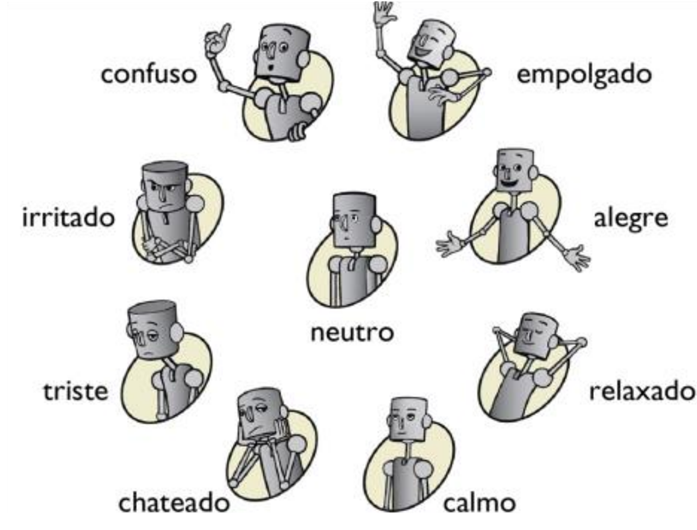
\includegraphics[width=0.8\textwidth]{Figuras/PAM.png}
\caption{Pick-A-Mood (PAM) \cite{santa2014teste}}
\label{fig:PAM}
\end{figure}

A Figura \ref{fig:PAM} apresenta a escala visual Pick-A-Mood (PAM), a qual é baseada em desenhos animados e que expressam oito tipos de humor, além do estado neutro. O humor é uma fonte de informações mais estável para o monitoramento emoções das pessoas sendo altamente relevante no design dada a sua capacidade de influenciar os comportamentos e atitudes, além de auxiliar as interações sociais como ser solidário com o próximo \cite{desmet2012pick}. No caso do jogo, além de mapear as emoções das crianças para constatar eventuais desconfortos que o jogo pudesse gerar (por ser um assunto delicado), é crucial observar a solidariedade manifestada pelas crianças no jogar do jogo. Entre os achado da pesquisa, grande parte das crianças manifestaram alegria e empolgação. Uma das crianças durante os experimentos relatou a emoção de tristeza. Tal emoção ocorreu em virtude de um personagem no jogo que manifestou os sintomas de um Acidente Vascular Cerebral, o que acaba por demostrar um sentimento de empatia e solidariedade por parte da criança. 

Como pode ser observado, existem pesquisas que se baseiam na construção de artefatos para desencadear certas emoções e pesquisas focadas na captação e interpretação mais assertiva destas informações. Com isso, espera-se ter construído um breve panorama de área de Design Emocional de Computação Afetiva. 


\section{Pesquisas em Aberto}\label{secao:desenvolvimento}

\citeonline{silva2019hold} apresentam o modelo \textit{\textbf{Hold Up}}, capaz de identificar situações de estresse e ansiedade, além da qualidade do sono por meio de sensores e realizar recomendações para auxiliar no aprimoramento do desempenho acadêmico de alunos. Algumas complicações são apresentadas pelo autores no que diz respeito aos experimentos realizados, deste modo, se torna mais do que necessária a execução uma pesquisa futura focada para validar ou confrontar os resultados na pesquisa realizada. Em adendo, os autores ressaltam a necessidade de uma identificação do emocional mais abrangente que proporcione constatar demais variáveis para serem trabalhadas, além das já englobadas por \citeonline{silva2019hold}.

\citeonline{moreira2019artefatos} se propuseram a desenvolver o \textit{software} \textit{\textbf{TangiSAM}}. A ideia do \textit{software} é a de efetuar uma avaliação de estados afetivos de maneira lúdica. Após a confecção do \textit{software}, o mesmo foi avaliado. A avaliação se deu para fornecer uma validação do \textit{software} proposto. Entre os achados foi constatado entre as crianças avaliadas que houve uma preferência delas pelo \textit{\textbf{TangiSAM}} quando comparado com outras propostas de representação de estados afetivos. O cronônimo final do nome (SAM) vem de Self-Assessment Manikin, uma modelo bastante conhecido na área de Iteração Humano-Computador (IHC). Os autores destacam a necessidade de aperfeiçoamento da ferramente proposta, algumas sugestões de melhorias são citadas, dentre elas está a necessidade de uma maneira para facilitar a avaliação simultânea em cenários com grandes quantidades de participantes. 

\citeonline{porsani2020ferramenta} desenvolveram o \textit{\textbf{EMOG}}, um sistema que trata a emoção por meio das relações semânticas de imagens e de escala de valoração. O \textit{\textbf{EMOG}} foi desenvolvido   no   formato   de   um   protocolo   eletrônico   digital, especificamente  elaborado  para  aplicação  na  Internet. No entanto, os autores relatam que novos estudos ainda devem ser conduzidos para contribuir com futuras investigações sobre a emoção na interação entre usuários e artefatos.

\citeonline{simacek2016design} tiveram como foco compreender as respostas emocionais de observadores de vitrinas, por meio de imagens das mesmas, aplicando metodologia observacional com o intuito de confrontar os dados nos âmbitos do emocional e de moda. Como resultado da pesquisa, foi concluído que a metodologia observacional traz resultados interessantes para o design emocional, a pesquisa foi realizada com um total de 154 participantes. Contudo, ainda é destacado pelos autores a necessidades de futuras pesquisas para se averiguar se objetos de design estudados estão adequados às necessidades psicológicas dos usuários no âmbito emocional. Em adendo, os autores ainda enfatizam o desenvolvimento de métodos específicos para pesquisas específicas, fugindo da ideia de aplicações e modelos genéricos na área do Design Emocional.


\section{Conclusão}\label{secao:conclusao}

Design Emocional é uma área que emergiu na década de 90, com o intuito de profissionalizar projetos com foco em emoção. Desde então, uma série de abordagens foram desenvolvida. Todas as abordagens descritas neste artigo podem ser úteis, dependendo da razão e da motivação do designer. Luzes, cores, formas, elementos tridimensionais encenam valores sociais, econômicos e culturais e isso provoca no observador uma mistura de sentimentos, sendo assim, questões estéticas, como a paleta de cores de um \textit{software} deve ser um assunto sério a ser levado em conta no momento de seu desenvolvimento. 

Ainda permanecem abertas inúmeras discussões sobre os modelos com foco nas emoções. Deste modo, também são poucos os estudos sobre como as emoções podem ser contempladas no processo de desenvolvimento de produtos. Assim como, não existem muitos modelos para contextos específicos na área do Design Emocional, sendo as exceções neste contexto alguns modelos da organização The Emotional Design Society da Universidadede Tecnologia de Delft.

O Design Emocional é uma área relativamente recente quando comparada com as demais. Em menos de 30 anos de área, o estudo das emoções do ponto de vista computacional já se demonstrou um grande diferencial. A juventude da área demarca inúmeras pesquisas futuras em potência, uma vez que grande parte do campo do Design Emocional ainda não tenha sido muito explorado. A tendência é que conforme o conhecimento da humanidade avance a área do Design Emocional cresça, garantindo cada vez mais, produtos agradáveis, amigáveis e que despertem emoções positivas e alegres as pessoas. 


\section*{Agradecimentos}\label{secao:agradecimentos}

O presente trabalho foi realizado com apoio da Coordenação de Aperfeiçoamento de Pessoal de Nível Superior - Brasil (CAPES) - Código de Financiamento 001.

%\bibliographystyle{sbc}
\bibliography{sbc-template}

\end{document}